\subsection{Coherent Light}

This section presents the experimental measurement of photon count distributions, which are used to infer Poissonian and super-Poissonian statistics.
Measurements were performed using the CW laser 1 (listed in section \ref{sec:lightsources}) in the following manner. 

\begin{itemize}
    \item Feed the CW laser 1 into the optical setup in figure \ref{fig:exp_lay}. 
    \item Mount Filter in between the source and the SPAD. 
    \item Set the integration time window to $100 \hspace{1mm} \mu s$ 
    \item Connect SPAD to Swabian Time Tagger. 
    \item Run the \texttt{tt.Counter} function and plot histogram. 
\end{itemize}

\begin{figure}[htpb]
    \centering
     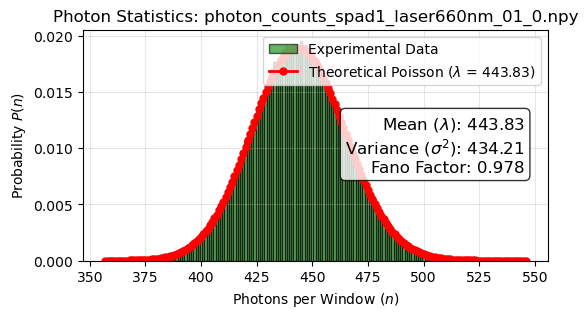
\includegraphics[width=0.5\textwidth]{Figures/photon_counts_spad1_01_0.png}
    \caption{Photon count distribution ($1 mW$).}
    \label{fig:photon_counts_spad1_01_0}
\end{figure}

\begin{figure}[htpb]
    \centering
     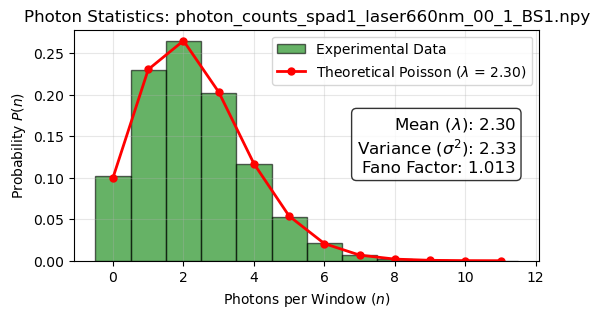
\includegraphics[width=0.5\textwidth]{Figures/photon_counts_spad1_00_1.png}
    %\rule{0.5\textwidth}{5cm}
    \caption{Photon count distribution($0.1 mW$).}
    \label{fig:photon_counts_spad1_00_1}
\end{figure}


As shown in Figure \ref{fig:photon_counts_spad1_00_1}, the coherent laser source yields a Poissonian distribution even as we vary the power of the CW laser.
Furthermore, in Figure \ref{fig:photon_counts_spad1_01_0}, a polarizing beam splitter was introduced to measure the curve in the low-power regime, also resulting in a Poissonian distribution.
The fact that the variance closely matches the mean ($\sigma^2 \approx \mu$) is consistent with the expected Poissonian statistics of coherent laser light. \\

\subsection{Non-Coherent Light}
We then replaced the light source with a fluorescent light bulb, acting as a non-coherent broadband source, and ran the previous experiment with the CW laser turned off. 
The resulting super-Poissonian distribution is shown in Figure \ref{fig:photon_counts_spad1_lablight}.

\begin{figure}[htpb]
    \centering
    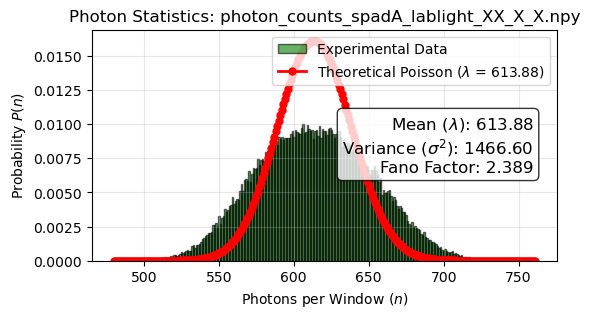
\includegraphics[width=0.5\textwidth]{Figures/photon_counts_spad1_lablight.png}
    %\rule{0.5\textwidth}{5cm}
    \caption{Photon counting statistics of the fluorescent light bulb, utilized here as a non-coherent broadband source. The experimental data follows a super-Poissonian distribution.}
    \label{fig:photon_counts_spad1_lablight}
\end{figure}
